\setchapterpreamble[u]{\margintoc}
\chapter{Validation} % Optimization strategy experimental validation
\labch{solhycool:validation}

\begin{kaobox}[title=To Do]
After the chapter is complete, find and replace all mentions to RBF, ANN, RMSE
and all other acronyms with the acronym with \Command{gls}.
\end{kaobox}

% ====================================
% ====================================
\section{Modelling}

The two main components of the system (\gls{wctLabel} and \gls{dcLabel}) are
modelled with different approaches and compared in detail. Afterward, the
integration of the selected modelling approach with the rest of the system
components (\refsec{cc:modelling:other-components}) is validated in
\nrefsec{cc:validation:complete-system}.

% \begin{enumerate}
% 	\item FP model
% 	\item DB from experimental campaign
% 	\item DB from FP
% 	\item Comparison
% \end{enumerate}


% ================================
\subsection{Wet cooler model alternatives comparison and validation}
\labsec{cc:validation:wct}

As previously mentioned\sidenote{See \nrefsec{cc:facility:exp-wct}}, three
experimental campaigns have been performed, shown in
\reffig{cc:validation:modelling:method} as \hyperref[sec:cc:facility:exp:1]{Exp
1}, \hyperref[sec:cc:facility:exp:2]{\hyperref[sec:cc:facility:exp:2]{Exp 2}},
and \hyperref[sec:cc:facility:exp:3]{\hyperref[sec:cc:facility:exp:3]{Exp 3}}.
\hyperref[sec:cc:facility:exp:1]{Exp 1} corresponds to the Poppe model
calibration campaign and it was designed for the calibration of the first
principles model. The aims of such campaign was to fit a function (mapping)
that relates the air mass flow rate at the outlet of the tower, $\dot{m}_a$,
with the frequency of the fan, $f_{fan}$:

\begin{figure}
  \includegraphics[]{figures/wascop-wct-exp-campaigns-diagram.png}
  \caption{Calibration, tuning, validation and comparison procedure}
  \labfig{cc:validation:modelling:method} 
\end{figure}

\begin{equation} 
    \dot{m}_a=-0.0014 f_{fan}^2+0.1743f_{fan}-0.7251.
    \labeq{cc:maffan} 
\end{equation}

and to calibrate a WCT performance coefficient: the Merkel number, $\Me$.
\reffig{cc:validation:Me_LG}\todo{Make text in figure larger} shows the
variation of the Merkel number as a function of the water-to-air mass flow
ratio ($\dot{m}_w/\dot{m}_a$) using data from
\hyperref[sec:cc:facility:exp:1]{Exp1}. As can be seen, the $\Me$ decreases
with $\dot{m}_w/\dot{m}_a$ values following a linear trend on log-log scale.   

% TODO: Make text in this figure larger
\begin{marginfigure}
    \includegraphics[width=1.1\linewidth]{figures/cc-poppe-Me_vs_mwma.png}
    \caption{Experimental results for the $\Me$ number as a function of $\dot{m}_w/\dot{m}_a$.}
    \labfig{cc:validation:Me_LG} 
\end{marginfigure}

Following the correlation for the Merkel number of a wet cooling tower
described in \refsec{cc:modelling:wct:poppe}, the parameters $c$ and $n$ obtained
from the data fitting are 1.516 and 0.693, respectively.

\subsubsection{Prediction capabilities}
Tabla tocha añadiendo casos (GPR, DD from FP, RF, GB)

The results of each modelling alternative and its comparison can be visualized
in \reffig{cc:validation:wct:prediction-comparison} and
\reftab{cc:validation:wct:results}. The results of each modelling alternative
and its comparison can be visualized
\reffig{cc:validation:wct:prediction-comparison} shows the results obtained
with the models using \hyperref[sec:cc:facility:exp:3]{Exp 3}. It shows the
perfect fit together with the results obtained with Poppe's model, MIMO FF,
cascade CF, and MIMO RBF. In \reftab{cc:validation:wct:results}, the
performance of the studied modelling approaches are included for the different
performance metrics\sidenote{Described in \refsec{intro:modelling:metrics}}.
\texttt{T} represents the performance metric value  for the training /
calibration dataset (\hyperref[sec:cc:facility:exp:1]{Exp 1} or
\hyperref[sec:cc:facility:exp:2]{Exp 2} depending on the case), and \texttt{V}
for the validation and comparison one (\hyperref[sec:cc:facility:exp:3]{Exp
3}). In all cases the model representing each alternative is in the best case
scenario, \ie maximum number of points available. On the other hand,
\texttt{s.u.} indicates that the units of the column are the same as from the
source variable.

% Gráfica hecha con: carpeta código/article_validation.m
\begin{figure}%
    % \centering
    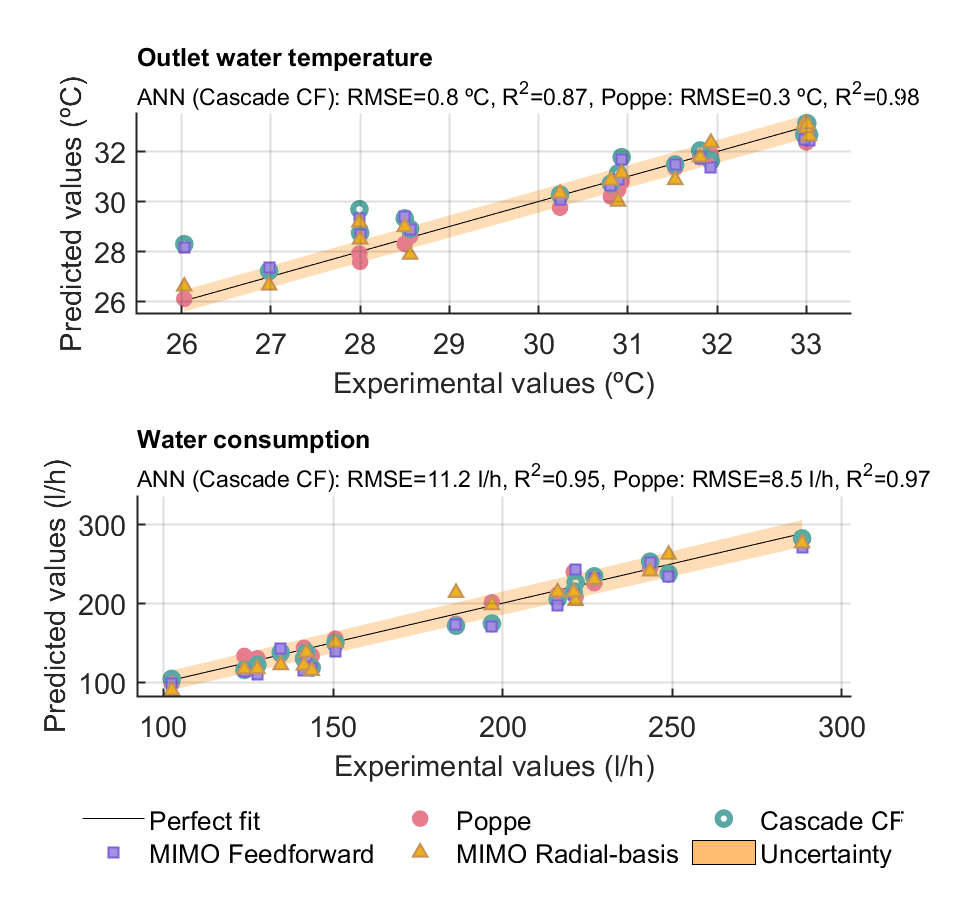
\includegraphics[width=\textwidth]{figures/cc-validation-comparison-models.eps}
    \caption{Model results obtained with Poppe and ANN models and data of \hyperref[sec:cc:facility:exp:3]{Exp3}}
    \labfig{cc:validation:wct:prediction-comparison}%
\end{figure}

Comparing both modelling approaches (see
\reffig{cc:validation:wct:prediction-comparison}), it can be outlined that both
models provide a good prediction of the output variables, falling most of the
discrepancies (errors) within the uncertainty range. Poppe's model provides a
better prediction of the outlet temperature, obtaining an RMSE of 0.33
$^\circ$C and an R$^2$ of 0.98. In comparison, the best ANN alternative (RBF
MIMO) has a slight worse performance with an RMSE of 0.51 $^\circ$C and
R$^2=0.95$. In terms of water consumption, the physical model has a better
prediction accuracy in terms of RMSE and  R$^2$ (8.5 l/h and 0.97) compared to
11.24 l/h and 0.95 for the best ANN model (cascade CF). It can be stated that,
although the results are better for the physical model (specially in the case
of the outlet temperature prediction), both approaches produce valid results
with high accuracy levels.

\begin{table*}[]
\caption{Summary table of the prediction results obtained with the different modelling approaches studied.}
\labtab{cc:validation:wct:results}
\resizebox{\linewidth}{!}{%
    
\begin{tabular}{cclccccccccccccccccccccccc}
\hline
\multicolumn{1}{c}{\multirow{3}{*}{\textbf{\begin{tabular}[c]{@{}c@{}}Predicted\\ variable\end{tabular}}}} & &
\multicolumn{1}{c}{\multirow{3}{*}{\textbf{\begin{tabular}[c]{@{}c@{}}Modelling\\ alternative\end{tabular}}}} & &
\multicolumn{1}{c}{\multirow{3}{*}{\textbf{\begin{tabular}[c]{@{}c@{}}Model\\ config\end{tabular}}}} & &
\multicolumn{1}{c}{\multirow{3}{*}{\textbf{\begin{tabular}[c]{@{}c@{}}Topology\end{tabular}}}} & &
\multicolumn{15}{c}{\textbf{Performance metric}} & &
\multicolumn{1}{c}{\multirow{3}{*}{\textbf{\begin{tabular}[c]{@{}c@{}}Evaluation\\ time (s)\end{tabular}}}} \\ 
\cline{9-23} \multicolumn{1}{c}{} & & \multicolumn{1}{c}{} & & & & & &
\multicolumn{3}{c}{\textbf{\begin{tabular}[c]{@{}c@{}}R$^2$\\ (-)\end{tabular}}} & &
\multicolumn{3}{c}{\textbf{\begin{tabular}[c]{@{}c@{}}RMSE\\ (s.u.)\end{tabular}}} & &
\multicolumn{3}{c}{\textbf{\begin{tabular}[c]{@{}c@{}}MAE\\ (s.u.)\end{tabular}}} & &
\multicolumn{3}{c}{\textbf{\begin{tabular}[c]{@{}c@{}}MAPE \\ (\%)\end{tabular}}} & &
\multicolumn{1}{c}{} \\
\cline{9-11} \cline{13-15} \cline{17-19} \cline{21-23}
\multicolumn{1}{c}{}  & & \multicolumn{1}{c}{}  & & \multicolumn{1}{c}{}  & & \multicolumn{1}{c}{}  & &
\multicolumn{1}{c}{T} & & \multicolumn{1}{c}{V} & &
\multicolumn{1}{c}{T} & & \multicolumn{1}{c}{V} & &
\multicolumn{1}{c}{T} & & \multicolumn{1}{c}{V} & &
\multicolumn{1}{c}{T} & & \multicolumn{1}{c}{V} & & \multicolumn{1}{c}{} \\
\cline{1-1} \cline{3-3} \cline{5-5} \cline{7-7} \cline{9-9} \cline{11-11} \cline{13-13} \cline{15-15} \cline{17-17} \cline{19-19} \cline{21-21} \cline{23-23} \cline{25-25}
\multirow{8}{*}{T$_{o,w}$ ($^\circ$C)}
    % Include Poppe manually
    & & Poppe & & - & & - & & - & & 0.98 & & - & & 0.33 & & - & & 0.27 & & - & & 0.87 & & 6.288 & \\
     & & Feedforward ANN & & MIMO & & 20-2 & & 0.93 & & 0.89 & & 0.52 & & 0.74 & & 0.37 & & 0.51 & & 1.22 & & 1.78 & & 0.004 & \\ & & Cascade-forward ANN & & MIMO & & 10-5-2 & & 0.93 & & 0.90 & & 0.50 & & 0.70 & & 0.35 & & 0.47 & & 1.15 & & 1.65 & & 0.004 & \\ & & Radial basis ANN & & MIMO & & 37-2 & & 0.99 & & 0.95 & & 0.23 & & 0.51 & & 0.18 & & 0.40 & & 0.57 & & 1.35 & & 0.004 & \\ & & Feedforward ANN & & Cascade & & 10-10-1 & & 0.94 & & 0.89 & & 0.46 & & 0.72 & & 0.32 & & 0.49 & & 1.05 & & 1.71 & & 0.007 & \\ & & Cascade-forward ANN & & Cascade & & 10-10-1 & & 0.94 & & 0.87 & & 0.46 & & 0.79 & & 0.31 & & 0.52 & & 1.02 & & 1.82 & & 0.008 & \\ & & Radial basis ANN & & Cascade & & 92-1 & & 0.99 & & 0.69 & & 0.23 & & 1.22 & & 0.08 & & 0.92 & & 0.25 & & 3.20 & & 0.008 & \\ \hline
\multirow{8}{*}{$\dot{m}_{w,lost}$ (l/h)}
    % Include Poppe manually
    & & Poppe & & - & & - & & - & &  0.97 & & - & & 8.47 & & - & & 6.74 & & - & & 3.74 & & 6.288 & \\
     & & Feedforward ANN & & MIMO & & 20-2 & & 0.95 & & 0.90 & & 11.75 & & 16.27 & & 9.47 & & 14.53 & & 7.74 & & 8.44 & & 0.004 & \\ & & Cascade-forward ANN & & MIMO & & 10-5-2 & & 0.96 & & 0.94 & & 10.52 & & 12.68 & & 8.23 & & 10.96 & & 6.68 & & 6.33 & & 0.004 & \\ & & Radial basis ANN & & MIMO & & 37-2 & & 0.99 & & 0.93 & & 4.88 & & 13.86 & & 3.67 & & 10.93 & & 2.94 & & 6.76 & & 0.004 & \\ & & Feedforward ANN & & Cascade & &  20-1 & & 0.97 & & 0.93 & & 9.64 & & 13.57 & & 7.50 & & 11.18 & & 6.12 & & 6.39 & & 0.007 & \\ & & Cascade-forward ANN & & Cascade & &  10-10-1 & & 0.97 & & 0.95 & & 8.52 & & 11.24 & & 6.18 & & 9.15 & & 4.92 & & 5.21 & & 0.008 & \\ & & Radial basis ANN & & Cascade & &  29-1 & & 0.98 & & 0.91 & & 7.63 & & 15.70 & & 4.54 & & 12.41 & & 4.13 & & 6.93 & & 0.008 & \\ \hline
\end{tabular}%
}
\end{table*}


\subsubsection{Experimental data requirements}

In order to estimate the minimum number of tests required to obtain
satisfactory results with both modelling strategies, an analysis was performed
in which each modelling alternative was calibrated/tuned for different case
studies with different amounts of available data, and then the performance
metrics were  evaluated. In this way, trends in the predictive accuracy of the
models as a function of the available data can be identified. When the
variation becomes small, it can be stated that the model has converged and
adding more information provides diminishing returns. 

For the physical model, the number of tests from Exp 1, used to calibrate $\Me$
correlation, was varied from 2 up to 16 data points added sequentially. In the
case of the ANN models, the available tuning data (Exp 2) was increased in
steps of 10 \%, starting from the availability of 10 \% up to the entire data
set (\mbox{100 \%}).

In both cases, the criteria for selecting the data was not random, but it was
done by applying physical knowledge. The water-to-air mass flow ratio,
$\dot{m}_w/\dot{m}_a $, is a good indicator for selecting the operation points
to be fed to the model. The trend observed in \reffig{cc:validation:Me_LG} (decreasing
Me for increasing $\dot{m}_w/\dot{m}_a $) has been extensively reported in the
literature. This behavior is explained by the increase in the amount of water
per unit of air that lead to a less effective cooling \sidecite{ruiz_thermal_2022}.
The situation corresponding to the minimum $\dot{m}_w/\dot{m}_a $ can be
interpreted as the maximum air flow rate for a given water flow rate to be
cooled. This results in the maximum driving force and, therefore, maximum
Merkel number. As $\dot{m}_a $ decreases progressively, the driving force
decreases for a given $\dot{m}_w $, and Me decreases accordingly. Based on this
knowledge, the selection starts by choosing extreme points for the water-to-air
mass flow ratio in the Me-$\dot{m}_a/\dot{m}_w$ relationship from the available
data, which gives information of the system operating in its limits.
Subsequently intermediate points are added, covering this way the whole
operating range of the cooling system.

\begin{figure}
    \includegraphics[width=\textwidth]{figures/wct-rmse-evolution.png}
    \caption{\gls{rmseLabel} evolution as a function of the number of points used for calibration/training of the Poppe's and data-driven approaches}
    \labfig{cc:wct:rmse-evolution}
\end{figure}

The results of this study are presented in \reffig{cc:wct:rmse-evolution}, where
the x-axis represents the number of available data points and the y-axis a
model performance metric (RMSE) obtained when the model outputs are compared to
data from Exp 3. From the results obtained, it can be clearly seen the
advantage of the physical model in terms of data requirements, since with the
minimal amount of points, good results are obtained, and by enlarging the
available data points to 8-10, low variation in the RMSE evolution can be
observed for both predicted variables. In the case of the ANN-based approaches,
the results differ depending on the ANN alternative. 

In terms of the outlet temperature, very good results (low error and variation)
are obtained with the minimal dataset (10 \% of available data, 12 data points)
for feedforward and cascade-forward in any configuration (MIMO and cascade). If
more data is added, RMSE is reduced from 1.1 up to 0.7 $^\circ$C. Although the
MIMO RBF outperforms the results of the other ANN alternatives, it does so only
from 90 points onwards. For this case, the downward trend is much more
noticeable but constant, which can not be stated for the cascade RBF,
displaying an erratic evolution up to 70 points. 

Similar conclusions can be drawn for the water consumption, except that in this
case the two RBF configurations achieve satisfactory results much earlier,
starting from 23 points.

Summarizing, both modelling approaches, Poppe's model and ANNs, produce
satisfactory results since their predictions fall well within the range of
uncertainty for all the case studies, although the obtained results, in terms
of RMSE, favor the physical model. Therefore, while the ANN model benefits from
as much data as possible, the Poppe model is already able to produce
satisfactory results with just two properly selected points. These two points
are easy to identify in advance because they are related to the maximum and
minimum $\dot{m}_w/\dot{m}_a$ ratio of the wet cooling tower. In practice, to
minimize the error prediction, around 5 points are often used. Out of the ANN
alternatives, considering both output variables, if less than 70 data points
are available, cascade-forward and feedforward alternatives with any
configuration are the best option, producing satisfactory results with as low
as 10 points. On the other hand, if enough data is available, MIMO RBF should
be considered as a strong candidate, but not in the cascade configuration
alternative.


\subsubsection{Sensitivity analysis}

\reminder{How to interpret \gls{saLabel} results}{ 
    The results are different sensitivity indices such as total sensitivity
    indices (total-order), first-order sensitivity indices (first-order), and
    interaction sensitivity indices (second-order). First-order measures the
    direct effect of an input variable on the output, excluding interaction
    effects with other variables, while the second-order measures specifically
    these interaction effects. Finally, total-order indices account for the
    total effect of an input variable, including both direct and interaction
    effects.\\
    More in \nrefch{intro:sa}. 
}

In \reffig{cc:validation:wct:sa}, only total-order sensitivity
indices\marginreminder{
    How to interpret \gls{saLabel} results}{ 
    The results are different sensitivity indices such as total sensitivity
    indices (total-order), first-order sensitivity indices (first-order), and
    interaction sensitivity indices (second-order). First-order measures the
    direct effect of an input variable on the output, excluding interaction
    effects with other variables, while the second-order measures specifically
    these interaction effects. Finally, total-order indices account for the
    total effect of an input variable, including both direct and interaction
    effects.\\
    More in \nrefch{intro:sa}. 
} are
represented in the y-axis for the two output variables (outlet temperature on
the top and water consumption on the bottom). Its value ranges from 0 to 1,
where 0 means the variable has no effect, and 1 means it has a significant
effect on the output\sidenote{values can go slightly above 1 due to computing
errors. This is due to the Sobol' sequence sample generator producing some
unfeasible test samples that need to be discarded}. The x-axis represents the
system's inputs and includes a bar for some of the obtained models with
different calibration or training data points. 

Comparing the results obtained for the different modelling approaches in
\reffig{cc:validation:wct:sa}, it can be seen that very homogeneous results are
obtained in all cases, except for the Cascade RBF case, which was the worst
performing of all the alternatives. These results serve to confirm that, at
least from a sensitivity analysis point of view, all valid approaches are
similarly sensitive to variations in the same inputs, which is desirable since
they are trying to predict the same physical system. In the case of Cascade
RBF,  a discrepancy can be observed; less relevant input variables ($T_{amb}$
and $\phi_{\infty}$) are overestimated and overall higher uncertainties in
sensitivity are observed.

It is also important to highlight that the observed results are in agreement
with the underlying physics of the heat and mass transfer processes occurring
in the exchange area of the tower. The frequency of the fan and the volumetric
flow rate are directly related to $\dot{m}_a$ and $\dot{m}_w$, respectively,
and they have a high influence on the heat transfer coefficients. These
coefficients govern the evaporation processes, which impact the evaporation
rate (water lost due evaporation) and the outlet water temperature. On the
other hand, the ambient conditions and the inlet water temperature also affect
the outputs, but less significantly, since the driving force for the
evaporation is the difference between the inlet air enthalpy and the enthalpy
of saturated air evaluated at water temperature.

\begin{figure}
    \includegraphics[width=\textwidth]{figures/wct-sensitivity_analysis.png}
    \caption{Sobol's sensitivity analysis result for different case studies}
    \labfig{cc:validation:wct:sa}
\end{figure}


% =================================
\subsection{Dry cooler model alternatives comparison and validation}

\subsubsection{Prediction capabilities}
Tabla tocha añadiendo casos (GPR, DD from FP, RF, GB)
La tabla debe incluir el tiempo de computación
\subsubsection{Experimental data requirements}
\subsubsection{Sensitivity analysis}

% =================================
\subsection{Complete system model validation}
\labsec{cc:validation:complete-system}


% A mi me gustaría que esta sección sea su propio capítulo
% Optimization validation
%================================
%================================
\section{Control and optimization results}

%================================
\subsection{Regular operation}
\labsec{solhycool:validation:regular-operation}

%================================
\subsection[Planned operation changes]{Planned changes in operation}
\labsec{solhycool:validation:planned-operation}

%================================
\subsection[Unanticipated operation changes]{Unanticipated operational changes}
\labsec{solhycool:validation:unanticipated-operation}